\section{Discussion}\label{sec:discussion}

\revisit{A similar equation for real space $E$ \& $B$ operators was derived in \cite{Zaldarriaga2001a}, however those results were derived for the flat sky case and did not explicitly derive the radial kernel.} \comment{A discussion on this should be in the conclusions.}

In this article we have cast the standard CMB polarization analysis operations in a vector matrix notation. Using this concise notation we derive the real space operators that translate the Stokes vector \vp{} to  the vector of scalars \vs and vice versa. We explicitly demonstrated that this real space operation can be simply interpreted as a convolution over the complex field $[Q - i U]$ (or $[E + iB]$) with an effective complex beam which is fully expressed in terms of the $Y_{\ell 2}$ spherical harmonic functions. We also use this vector matrix notation to derive real space operators which allow the direct decomposition of the full Stokes vector \vp{} into the vector \vp{E} and \vp{B} that correspond to the respective scalar modes. 

Given the effective beam interpretation of these real space operators we derive the harmonic coefficients of these effective beams at the north galactic pole. Using these harmonic coefficients we provide a prescription for computing the convolution kernels at any position on the sphere using the standard Healpix built in functions. The procedure is equivalent to parallel transporting the beam at the north pole to any desired location on the sphere. We implement the prescription to compute the  kernel at different location on the sphere and provide simple explanations in terms of Euler angles for the observed variations.

These real space convolution kernels provide a spatially intuitive way of understanding the construction of the scalar modes. We explicitly show that the kernels separates into an band limit independent azimuthal operation around any given direction which is primarily responsible for requisite decomposition, while the band limit dependent radial weights can be interpreted as some isotropic smoothing operation. These radial weights primarily determine the non-local dependence of the construction of the respective fields at any location on the Stoke field. We define the parameter $\beta_0$ as a means to characterize the non-locality and show that $\beta_0$ scales $\propto \ell_{\rm max}^{-1}$. We show that this non-locality parameter also characterized the non-locality of the $\bar{O}_{E/B}$ operators. 

Finally we present the generalized real space operators $\bar{O}'$, which are derived by allowing the radial function to vary from its default form. We derive constraints on the modifications to these radial function by demanding the inverse operator to be well defined. We argue that these modifications to the radial kernel can be be interpreted as a some smoothing smoothing operation on the scalar fields with a circularly symmetric instrument beam. We also show that as long as these radial function are invertible, the standard spectra can always be recovered from these modified $E'$ \& $B'$ maps. The main advantage of modifying these radial function is the ability to generate more locally defined $E$ and $B$ mode maps. This could potentially be useful in reducing foreground contamination on large angular scales in a full sky $E/B$ analysis. Also defining more locally constructed scalar fields $E$ \& $B$ can be used to circumvent the power leakage nuisance. We explore and demonstrate the working of these ideas in the next paper in this series. 
%\revisit{The discussion till now gives the impression that using the localized convolution kernels is no different from from using the default kernel and altering the spherical harmonic coefficients of expansion of the relavant fields by appropriately operating on them with the  effective beam functions $g_{\ell}$. To appreciate the difference between these two, it is important to realize that in general one can make a choice of a radial function which may not have a band limited description. In such a case these two method of evaluating the relevant fields is not identical. An example of this claim is depicted in \fig{fig:example_gbeta}.\\
%Another important thing to realize is that the harmonic coefficients derived from default full sky operations get some contributions from different portions of sky. For instance evaluating the E and B fields in the vicinity of the poles is are prone to receiving significant contributions from strong foregrounds near the equator. Correcting the harmonic coefficients of expansion with the effective beam function does not cancel these non-local contribution. On the contrary by performing the convolution with the localized real space kernels, the regions which contribute to the local field evaluations are predetermined by the choice of the radial function.}


\section{Understanding polarization signatures of magnetized filaments}
\label{sec:pol_filaments}

The real space kernels give us a better intuitive understanding of the $E/B$ modes associated with physical objects.  For example, a simple model for a magnetized filament has the magnetic field threaded along a linear gas over-density.  Precession of the dust grains around the magnetic field leads to a net polarization perpendicular to the magnetic field (and perpendicular to the filament overall).  For a filament aligned North--South, the polarization will be horizontal or $Q<0$, $U=0$ (left pane of \fig{fig:polfilaments}).  The Green's function kernels for horizontal polarization are rotated by 90 degrees relative to the components of $\cal{M}_G$ in \fig{fig:vis_kernel}.

The kernel can be thought of as the orientable nib of a calligraphy pen or paintbrush that we can trace along the filament.  The positive components for the $E$ part of the Green's function align and reinforce along the filament, consequently the filament is highlighted as a segment with $E>0$.  Since the over-density will also have emission in total intensity, this naturally predicts a positive $TE$ correlation for magnetized filaments.  The $E$ pattern is somewhat negative along the outside of the filament, also a consequence of the kernel shape.

The $B$ part of the Green's function, traced along the filament, cancels itself except at the filament ends.  This results in a non-zero $B$ pattern for the filament.  For a North--South filament, the $B$-mode pattern is positive on the North-East and South-West, and negative in the North-West and South-East as seen in \fig{fig:polfilaments}.  The size of this $B$-mode pattern is set by the dimensions of the filament, chiefly the width.  In contrast to the kernel radial fuctions, which are more compact at higher band limit, the filament $B$-mode  pattern does not depend much on the band limit, provided it is sufficient to resolve the filament structure.  A filament with a more gradual edge has a $B$-pattern that is more spread out, but follows the same general structure.

The non-zero $B$ result is somewhat surprising given that the polarization pattern is symmetric to both horizontal and vertical reflections through the filament center.  However, unlike a circular ring, this filament is not a configuration with a definite parity.  Since the scalar description of polarization is coordinate independent, the $E/B$ patterns do not depend on the orientation of the filament.  For example, a filament inclined at $45^\circ$ will have a similarly inclined $E/B$ pattern, but different reflection symmetries.  

Changing the polarization direction within the filament changes the $E/B$ patterns.  A $90^\circ$ rotation of the polarization with respect to the filament changes the sign of both $E$ and $B$.  In a polarization pattern aligned at $45^\circ$ to the filament, the $E$ pattern will swap with the $B$ pattern.  The work in \cite{Zaldarriaga2001a} correctly argued that linear filaments (infinite and without ends) can only produce $E$-power, but we find that for realistic filaments, the ends produce $B$-mode power with a clear signature.  Careful study of the $E/B$ mode power in filaments can provide insights into the orientation of the magnetic field with respect to the axis of the filament, this information could potentially shed light on the internal dynamics of filaments.
% 
\begin{figure}[t]
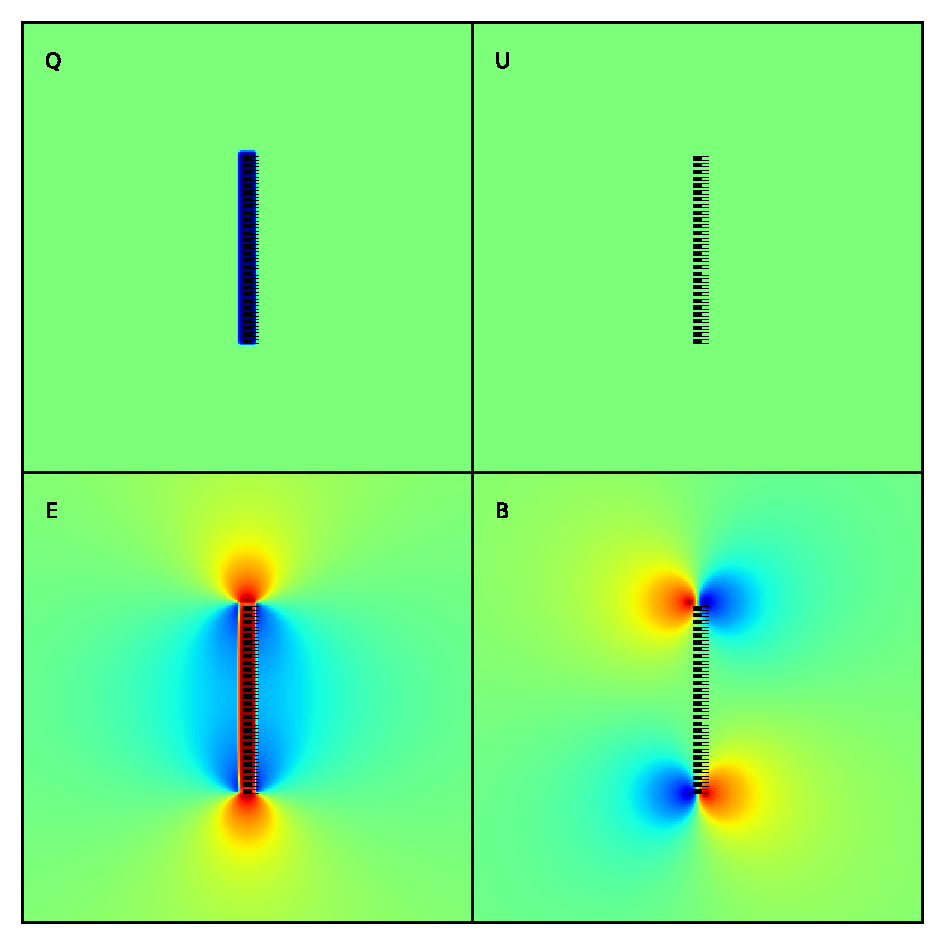
\includegraphics[width=0.5\columnwidth]{line.pdf}
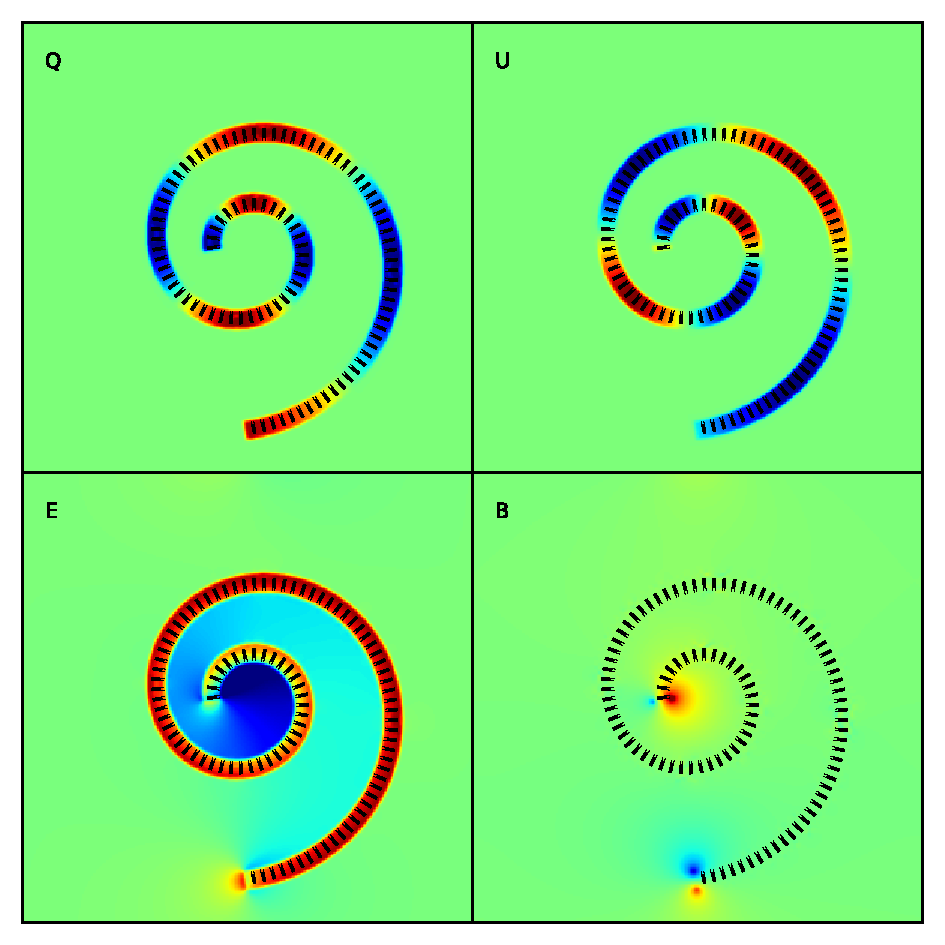
\includegraphics[width=0.5\columnwidth]{spiral.pdf}
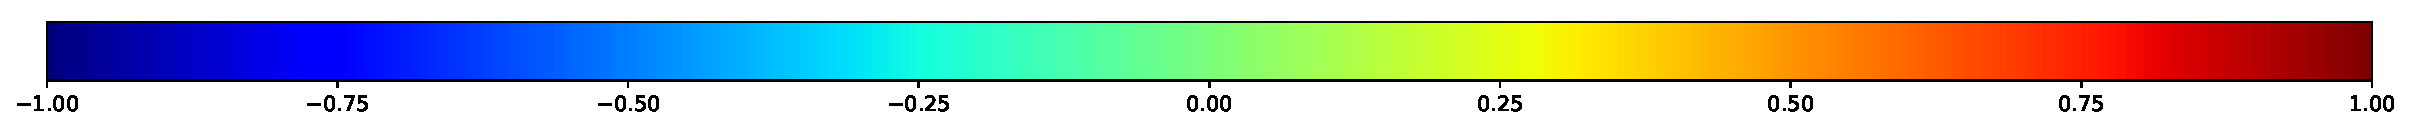
\includegraphics[width=1.0\columnwidth]{colorbar.pdf}
\caption{ The polarization signals of toy filament structures. In a filament organized perfectly along a magnetic field line, the polarization will be perpendicular to the filament direction.  The $E/B$ modes of filaments are in some ways easier to think about than the Stokes parameters. Left panels: in a straight filament, the $E$-mode is positive along the filament and at the ends, but negative along the sides.  The $B$-modes are only non-zero at the ends.  Right panels: in a curved filament, the $E$-mode is again positive along the filament.  Outside the filament, the $E$-mode is more negative on the interior of the curve than the exterior.  The $B$-modes are again non-zero at the ends, akin to the straight filament case, but also somewhat along the filament due to the changing radius of curvature. In all images, the longitude angle increases to the left (which is East in sky convention).  All plot are on a common, arbitrary color scale.}
\label{fig:polfilaments}
\end{figure}
%
\indent The intuition from the real-space kernels holds also when we distort the shape of the filament.  If the filament were bent around into a circle, the positive and negative parts of the $B$ pattern will cancel, and we are left with a hoop of pure $E$ pattern. Here it is important to note that this cancellation will not happen for an ellipse or any loop of non-constant radius of curvature.
The same general description holds for a spiral-shaped filament, which can can be viewed as distortion of the straight filament (right panel of  \fig{fig:polfilaments}).  The filament is highlighted by positive $E>0$.  The $E$-pattern is more negative on the interior of a curve than on the exterior, and the concentric rings of filamentary structure make an increasingly negative $E$ value inside. While the $B$-pattern is again concentrated at the ends of the filament in an oriented pair of positive/negative fluctuations, note that it is non-vanishing in the intermediate regions along the filament due to the varying radius of curvature of the spiral.  A spiral turning with the other handedness will have a $B$-pattern with the opposite sign.

A stacking analysis of Planck data \citep{2016A&A...586A.141P} sees $E>0$ along filaments (selected from intensity data), but claims no $B$-mode signal above the noise. We predict that a $B$-mode signal from filaments should be present, since they have a finite length of a few degrees.  Detecting $B$-modes from filaments will be easier with more signal-to-noise and may require a more careful filament analysis, rescaling and aligning the filament ends.  While the detectability of the $B$-mode signature from stacked filaments in Planck data calls for a more careful assessment, we should see it in higher-fidelity data. 


